\section{Nedeterministické konečné automaty}\label{sec:nedet-automaty}

U~deterministického automatu vede pro daný stav a~znak nejvýše jeden přechod. Někdy je však návrh mnohem jednodušší,~když automatu dovolíme několik možností a~představíme si,~že vyzkouší všechny paralelně.

\begin{definition}[Potenční množina]
    Nechť $M$ je množina. \emph{Potenční množinou} množiny $M$ nazveme množinu všech jejích podmnožin. Značíme ji
    \[
        \powset{M}=\set{N:N\subseteq M}.
    \]
    Například pro $M=\set{q_0,q_1}$ dostaneme
    \[
        \powset{M}=\set{\emptyset,\set{q_0},\set{q_1},\set{q_0,q_1}}.
    \]
\end{definition}

\begin{definition}[Nedeterministický konečný automat]
    \emph{Nedeterministický konečný automat} (zkráceně NFA) je pětice
    \[A=(Q,\Sigma,\delta,q_0,F),\]
    kde $Q$,~$\Sigma$,~$q_0$ a~$F$ mají stejný význam jako u~DFA a
    \[\delta:Q\times\Sigma\to\powset{Q}\]
    přiřazuje dvojici stavu a~znaku množinu možných následujících stavů.
\end{definition}

Přečte-li NFA ve stavu $q$ znak $a$,~výpočet se rozvětví do všech stavů z~$\delta(q,a)$. Je-li tato množina prázdná,~daná větev zanikne. Automat přijme vstupní slovo právě tehdy,~když \emph{alespoň jedna} větev po přečtení celého slova skončí v~přijímajícím stavu.

\begin{example}[Slova obsahující podslovo $101$]\label{ex:nfa-101}
    Počáteční stav $q_0$ zpracovává libovolný začátek slova. Při každé jedničce může automat zároveň \uv{uhádnout},~že právě začalo hledané podslovo,~a~spustit novou větev ve stavu $q_1$.
    \begin{figure}[h]
        \centering
        \begin{tikzpicture}
    \initialstate{q0}{(0,0)}{$q_0$}{(-1.2,0)}{180}
    \state{q1}{(2.4,0)}{$q_1$}
    \state{q2}{(4.8,0)}{$q_2$}
    \acceptingstate{q3}{(7.2,0)}{$q_3$}
    \transitionarrow[loop above]{q0}{above}{$0,1$}{q0}
    \transitionarrow{q0}{above}{$1$}{q1}
    \transitionarrow{q1}{above}{$0$}{q2}
    \transitionarrow{q2}{above}{$1$}{q3}
    \transitionarrow[loop above]{q3}{above}{$0,1$}{q3}
\end{tikzpicture}

        \caption{NFA přijímající právě slova obsahující podslovo $101$.}
        \label{fig:nfa-101}
    \end{figure}
    Pro slovo $01101$ vznikne přijímající větev,~která po posledních třech znacích projde stavy $q_1,q_2,q_3$.
\end{example}

\begin{example}[Třetí znak od konce je $1$]\label{ex:nfa-treti-od-konce}
    NFA může při každé přečtené jedničce odhadnout,~že do konce zbývají právě dva znaky. Pak už pouze odpočítá dva další přechody.
    \begin{figure}[h]
        \centering
        \begin{tikzpicture}
    \initialstate{q0}{(0,0)}{$q_0$}{(-1.2,0)}{180}
    \state{q1}{(2.5,0)}{$q_1$}
    \state{q2}{(5,0)}{$q_2$}
    \acceptingstate{q3}{(7.5,0)}{$q_3$}
    \transitionarrow[loop above]{q0}{above}{$0,1$}{q0}
    \transitionarrow{q0}{above}{$1$}{q1}
    \transitionarrow{q1}{above}{$0,1$}{q2}
    \transitionarrow{q2}{above}{$0,1$}{q3}
\end{tikzpicture}

        \caption{NFA pro jazyk slov,~jejichž třetí znak od konce je $1$.}
        \label{fig:nfa-treti-od-konce}
    \end{figure}
    Tento automat má jen čtyři stavy. Ekvivalentní DFA si musí pamatovat všechny možné konce délky tři a~potřebuje osm stavů.
\end{example}

\begin{example}[Jednoduchý zápis desetinného čísla]
    Automat na obrázku \ref{fig:automat-desetinne} přijímá neprázdný blok číslic a~případně desetinnou tečku následovanou dalším neprázdným blokem číslic. Přijme tedy \texttt{17} a~\texttt{17.25},~ale odmítne \texttt{.25},~\texttt{17.} i~\texttt{1.2.3}.
    \begin{figure}[h]
        \centering
        \begin{tikzpicture}
    \initialstate{s}{(0,0)}{$s$}{(-1.2,0)}{180}
    \acceptingstate{i}{(2.5,0)}{$q_i$}
    \state{dot}{(5,0)}{$q_t$}
    \acceptingstate{f}{(7.5,0)}{$q_f$}
    \transitionarrow{s}{above}{$0,\dots,9$}{i}
    \transitionarrow[loop above]{i}{above}{$0,\dots,9$}{i}
    \transitionarrow{i}{above}{\texttt{.}}{dot}
    \transitionarrow{dot}{above}{$0,\dots,9$}{f}
    \transitionarrow[loop above]{f}{above}{$0,\dots,9$}{f}
\end{tikzpicture}

        \caption{Konečný automat pro jednoduchý zápis nezáporného desetinného čísla.}
        \label{fig:automat-desetinne}
    \end{figure}
\end{example}

\subsection{Vztah DFA a~NFA}

Nedeterminismus sice může výrazně zjednodušit zápis automatu,~ale nerozšíří množinu jazyků,~které konečné automaty dokážou přijímat.

\begin{theorem}[Podmnožinová konstrukce]\label{thm:subset-construction}
    Ke každému NFA $A$ existuje DFA $B$ takový,~že $L(A)=L(B)$.
\end{theorem}
\begin{proof}
    Mějme NFA $A=(Q,\Sigma,\delta,q_0,F)$. Jeden stav nového DFA bude popisovat celou množinu stavů,~v~nichž se NFA může po přečtení stejného začátku slova nacházet. Položíme tedy
    \[B=(\powset{Q},\Sigma,\delta',\set{q_0},F'),\]
    kde
    \[\delta'(S,a)=\bigcup_{q\in S}\delta(q,a)\]
    a~množina $S\subseteq Q$ je přijímajícím stavem právě tehdy,~když $S\cap F\neq\emptyset$.

    Indukcí podle délky přečteného slova dostaneme,~že stav DFA $B$ je vždy přesně množinou všech stavů,~ve kterých mohou být jednotlivé větve NFA $A$. DFA proto přijme právě tehdy,~když alespoň jedna větev NFA skončí v~$F$.
\end{proof}

Každý DFA je zároveň NFA,~jen všechny množiny $\delta(q,a)$ mají nejvýše jeden prvek. Oba modely tedy přijímají stejné jazyky. Cena za odstranění nedeterminismu může být vysoká: NFA s~$n$ stavy může podmnožinovou konstrukcí vytvořit DFA až s~$2^n$ stavy.

\subsection{Přechody bez čtení znaku}

Pro důkaz Kleeneho věty se nám bude hodit ještě drobné technické rozšíření.

\begin{definition}[$\lambda$-NFA]
    \emph{$\lambda$-NFA} je NFA s~přechodovou funkcí
    \[
        \delta:Q\times(\Sigma\cup\set{\lambda})\to\powset{Q},
    \]
    který smí navíc použít přechod označený $\lambda$. Při takovém přechodu změní stav,~aniž by přečetl znak vstupu.
\end{definition}

Takový automat stále nepřijímá nic navíc. Pro množinu stavů $S$ označme $E(S)$ množinu všech stavů dosažitelných ze $S$ pouze pomocí nulového nebo více $\lambda$-přechodů. Obyčejný NFA sestrojíme tak,~že pro každý stav $q$ a~znak $a$ položíme
\[\delta'(q,a)=E\left(\bigcup_{r\in E(\set{q})}\delta(r,a)\right)\]
a~stav $q$ prohlásíme za přijímající,~pokud $E(\set{q})\cap F\neq\emptyset$. Nový automat před každým znakem i~po něm provede předem všechny možné $\lambda$-přechody,~takže přijímá tentýž jazyk.

\subsection{Regulární jazyky}

\begin{definition}[Regulární jazyk]
    Jazyk $L$ nazveme \emph{regulární},~pokud existuje DFA $A$ takový,~že $L=L(A)$.
\end{definition}

Podle věty \ref{thm:subset-construction} můžeme v~definici stejně dobře použít NFA nebo $\lambda$-NFA. Ne každý jazyk je však regulární.

\begin{theorem}\label{thm:leq-neregular}
    Jazyk
    \[L_{\mathrm{eq}}=\set{w\in\set{0,1}^*:|w|_0=|w|_1}\]
    není regulární.
\end{theorem}
\begin{proof}
    Předpokládejme pro spor,~že existuje DFA $A$ s~$m$ stavy a~$L(A)=L_{\mathrm{eq}}$. Uvažujme $m+1$ slov
    \[\lambda,0,00,\dots,0^m.\]
    Automat má jen $m$ stavů,~takže po přečtení dvou různých slov $0^i$ a~$0^j$,~kde $0\leqslant i<j\leqslant m$,~musí být ve stejném stavu.

    Nyní k~oběma slovům připojme stejný konec $1^i$. Automat z~téhož stavu čte tentýž zbytek,~a~proto buď přijme obě slova,~nebo obě odmítne. Jenže
    \[0^i1^i\in L_{\mathrm{eq}},\qquad 0^j1^i\notin L_{\mathrm{eq}}.\]
    Automat by je musel rozlišit. Dostáváme spor.
\end{proof}

\begin{figure}[h]
    \centering
    \begin{tikzpicture}[node distance=18mm]
    \node[task] (a) {$0^i$};
    \node[task,below=12mm of a] (b) {$0^j$};
    \state{q}{(3.3,-0.65)}{$q$}
    \acceptingstate{f}{(6.6,-0.65)}{$f$}
    \draw[diredge] (a) -- node[above,sloped]{čtení} (q);
    \draw[diredge] (b) -- node[below,sloped]{čtení} (q);
    \transitionarrow{q}{above}{$1^i$}{f}
    \node[below=8mm of f] {$0^i1^i\in L_{\mathrm{eq}}$, ale $0^j1^i\notin L_{\mathrm{eq}}$};
\end{tikzpicture}

    \caption{Po slovech $0^i$ a~$0^j$ je automat ve stejném stavu,~takže stejný konec $1^i$ už nedokáže rozlišit.}
\end{figure}
